% \begin{itemize}
%     \item Using the runtime portion of the data you collected during the performance runs, produce a speedup chart showing the scaling performance of your BMMCO-omp code across all levels of concurrency and problem sizes in this assignment. This will be a single chart containing 6 datasets: three concurrency levels,  t=4,16,64, and two block sizes, b=4,16.
%     \item Discuss the performance of your BMMCO-omp code across the set of problem sizes, block sizes, and concurrency levels. Describe how speedup changes as a function of problem size, and give an explanation as to why you think that change occurs. 
% \end{itemize}

The scaling performance of the BMMCO OMP implementation was analyzed across different concurrency levels (\(p = 4, 16, 64\)), block sizes (\(b = 4, 16\)), and matrix sizes (\(N = 128, 512, 2048\)). Figure~\ref{fig:blocked-speedup} presents the speedup chart for six different configurations, illustrating the interplay between concurrency levels, block sizes, and problem sizes.

Overall, the scaling behavior aligns well with Amdahl's Law \cite{amdahl1967validity}, with larger matrix sizes yielding near-ideal speedup as parallelism increases. Larger problem sizes effectively reduce the overhead from serial portions of the code and allow for more efficient workload distribution across threads.

One notable observation is that a block size of 4 achieved better speedup for smaller matrix sizes (\(N = 128, 512\)) compared to a block size of 16. Specifically, Blocked B16 at concurrency levels of \(p = 16, 64\) for \(N = 128\) and \(p = 64\) for \(N = 512\) exhibited limited speedup. Additionally, Blocked B4 for \(N = 128\) showed that increasing the thread count from \(p = 16\) to \(p = 64\) actually resulted in worse performance. These observations can be attributed to how parallelism was applied in the BMMCO implementation, where the outermost loop was parallelized (as shown in Listing~\ref{listing:BMMCO-omp}). The number of iterations in this outermost loop corresponds to the number of blocks along a row, which directly affects thread utilization.

Tables~\ref{tab:b4-threads-utilization} and \ref{tab:b16-threads-utilization} show the number of blocks per row for different matrix sizes and block sizes, along with the corresponding thread utilization for different concurrency levels. For \(b = 16\) and \(N = 128\), only 8 blocks are available, which limits the number of threads that can be effectively utilized to 8. This is significantly lower than the total available threads for configurations with \(p = 16, 64\), leading to underutilization of potential parallelism. Similarly, for \(N = 512\), \(b = 16\) results in 32 blocks, which limits effective thread utilization to 32 when using \(p = 64\).

On the other hand, \(b = 4\) provides more blocks for each problem size, which enables better thread utilization, particularly for smaller matrices like \(N = 128\). For \(N = 128\), \(b = 4\) allows for 32 blocks, which is sufficient to fully utilize threads for configurations with \(p = 4, 16\). However, increasing the thread count to \(p = 64\) resulted in underutilization, as the overhead of multithreading outweighed the performance gain from adding more threads. 

In conclusion, block size has a significant impact on scaling performance, particularly for smaller problem sizes. The availability of sufficient blocks to match the number of threads determines the efficiency of parallelism. For larger matrices (\(N = 2048\)), both block sizes showed good scalability, as there were enough blocks available to fully utilize all threads across all concurrency levels.

\begin{figure}[htbp]
    \centering
    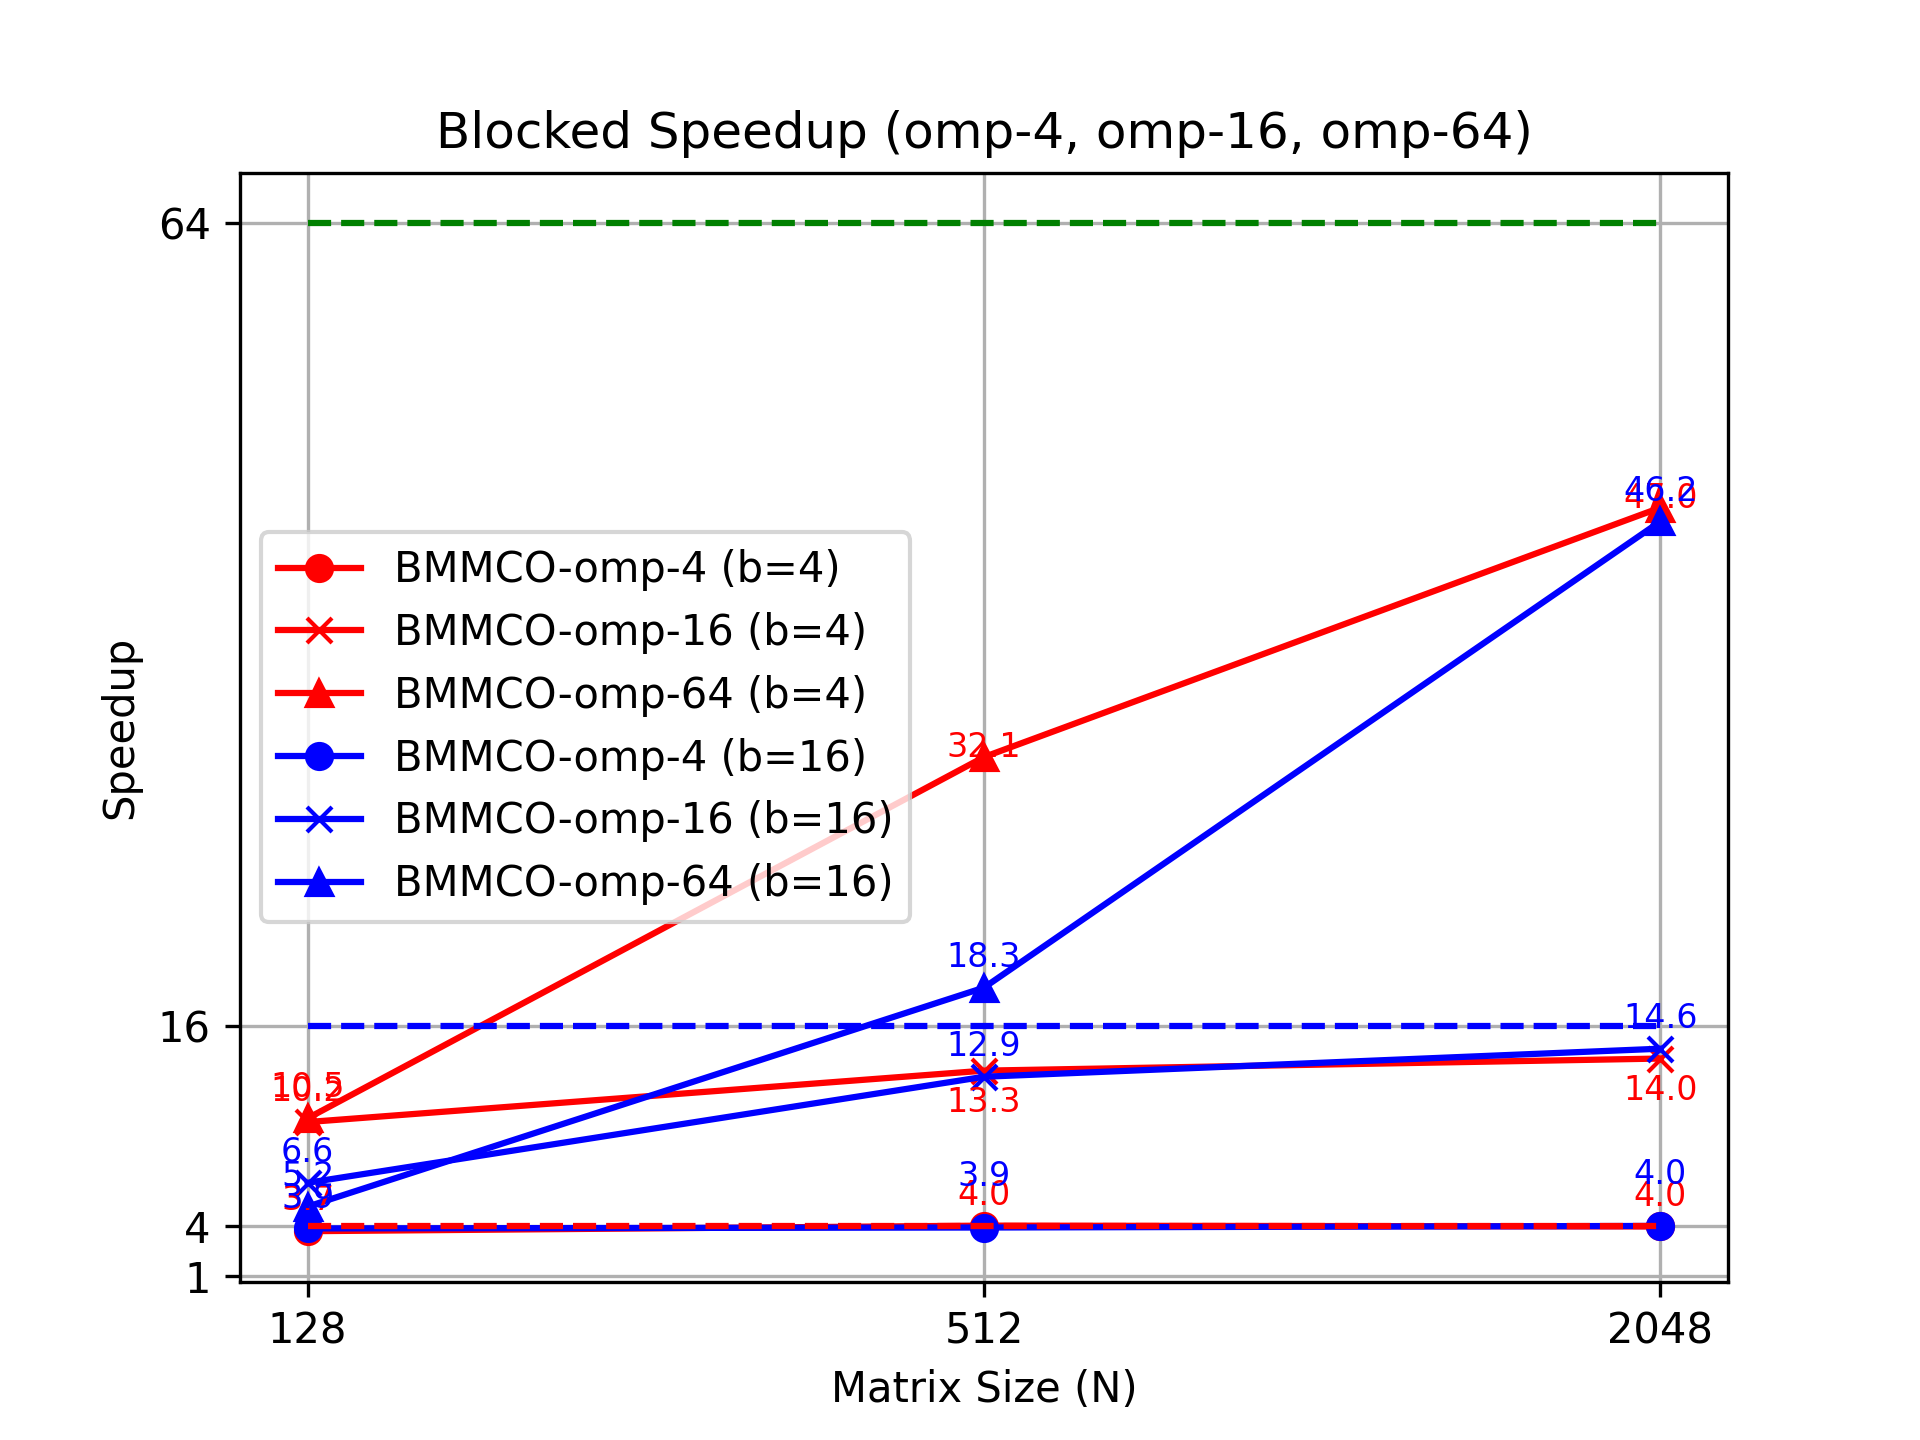
\includegraphics[width=1.0\linewidth]{images/Blocked_Speedup.png}
    \caption{\textbf{Speedup of BMMCO with OpenMP Parallelization for Different Block Sizes.} The figure shows the speedup achieved by the BMMCO implementation at different concurrency levels (\(p = 4, 16, 64\)) for matrix sizes of \(N = 128, 512, 2048\) with block sizes of \(b = 4\) and \(b = 16\). The results demonstrate that \(b = 4\) generally provides better performance for smaller matrix sizes due to improved thread utilization, whereas \(b = 16\) struggles to fully leverage available threads for smaller matrices.}
    \label{fig:blocked-speedup}
\end{figure}

\begin{table}[htbp]
    \centering
    \begin{tabular}{lrrrr}
    \toprule
    N & Blocks & \(p=4\) & \(p=16\) & \(p=64\) \\
    \midrule
    128  & 32 & 100\% & 100\% & 50\% \\
    512  & 128 & 100\% & 100\% & 100\% \\
    2048 & 512 & 100\% & 100\% & 100\% \\
    \bottomrule
    \end{tabular}
    \caption{\textbf{Number of Blocks per Row and Thread Utilization for Block Size of 4.} The table shows the number of blocks per row for different matrix sizes and the resulting thread utilization percentage for different concurrency levels. Block size \(b = 4\) provides sufficient blocks to maintain high thread utilization for most configurations.}
    \label{tab:b4-threads-utilization}
\end{table}

\begin{table}[htbp]
    \centering
    \begin{tabular}{lrrrr}
    \toprule
    N & Blocks & \(p=4\) & \(p=16\) & \(p=64\) \\
    \midrule
    128  & 8 & 100\% & 50\% & 12.5\% \\
    512  & 32 & 100\% & 100\% & 50\% \\
    2048 & 128 & 100\% & 100\% & 100\% \\
    \bottomrule
    \end{tabular}
    \caption{\textbf{Number of Blocks per Row and Thread Utilization for Block Size of 16.} The table shows the number of blocks per row for different matrix sizes and the resulting thread utilization percentage for different concurrency levels. Block size \(b = 16\) results in fewer blocks for smaller matrices, which limits the effective thread utilization, particularly at higher concurrency levels.}
    \label{tab:b16-threads-utilization}
\end{table}
